\documentclass[12pt,handout,notes=on]{beamer}
\usepackage[italian]{babel}
\usepackage[utf8]{inputenc}
\usepackage[T1]{fontenc}
\usepackage{xcolor}
\usepackage{fancyhdr}
\usepackage{amsthm}
\usepackage{amsmath}
\usepackage{amssymb}
\usepackage{lmodern}
\usepackage{tikz}

%\usepackage{SIunits}

\usepackage[]{hyperref}

\usetikzlibrary{decorations}
%\usetikzlibrary{snakes}

\title{Corso di Introduzione all'Elettronica}
\author[Alja\v{z}, Ruggero]{Alja\v{z} Srebrni\v{c} \and Ruggero Lot}
\date[23/5]{Maggio 2015}
\institute[Mittelab]{Mittelab}
\logo{\includegraphics[scale=0.07]{./img/mittelab.pdf}}
\usetheme{Rochester}
%\useoutertheme[infolines]{}
\setbeamercovered{dynamic}

\begin{document}
	
	\begin{frame}[c]\frametitle{}
		\maketitle
	\end{frame}

	\begin{frame}\frametitle{Piano della presentazione}
		\tableofcontents	
	\end{frame}
	\note{Noi volgiamo partire da una base molto semplice di struttura della materia per capire cosa genera in realtà questa corrente e riuscire ad immaginarci un po' cosa sta accadendo
prima di thompson non si pensava che l'atomo fosse un unità indivisibile poi invece tutto cambi}

	\section{Storia} % (fold)
	\label{sec:storia}
	
	\begin{frame}[t]\frametitle{Storia}
		\begin{itemize}
			\item 1897 $\longrightarrow$ \href{http://www.wired.it/scienza/energia/2014/04/30/la-scoperta-dellelettrone/}{Scoperta dell'elettrone} da parte di Thompson 
			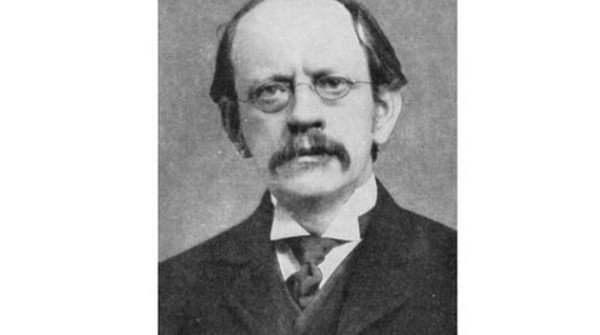
\includegraphics[width=4cm]{./img/thompson.jpg}
			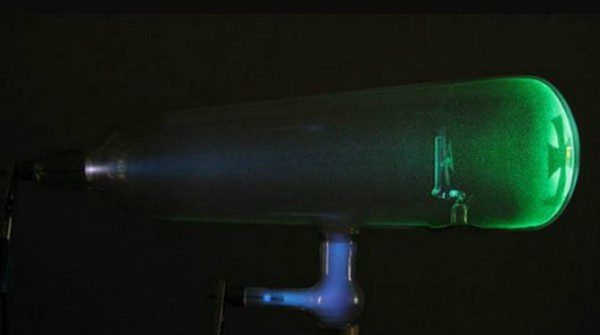
\includegraphics[width=4cm]{./img/tubo.jpg}
			\pause
			\item 1900  $\longrightarrow$ Primo modello di metallo proposto da Paul Drude (1863 – 1906) con l' \href{http://www.dmf.unicatt.it/~sangalet/PLS/Buone_pratiche/Esperimento_Rutherford.pdf}{atomo a panettone}
			%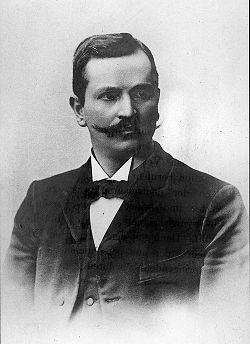
\includegraphics[width=2cm]{./img/Drude.jpg}
			\pause
			\item 1911  $\longrightarrow$ Atomo di Ernest Rutherford ( 1871 – 1937)
		\end{itemize}
	\end{frame}

	\begin{frame}[c]\frametitle{Atomo di Rutherford}
	    
		\begin{figure}[tb]
			\centering
			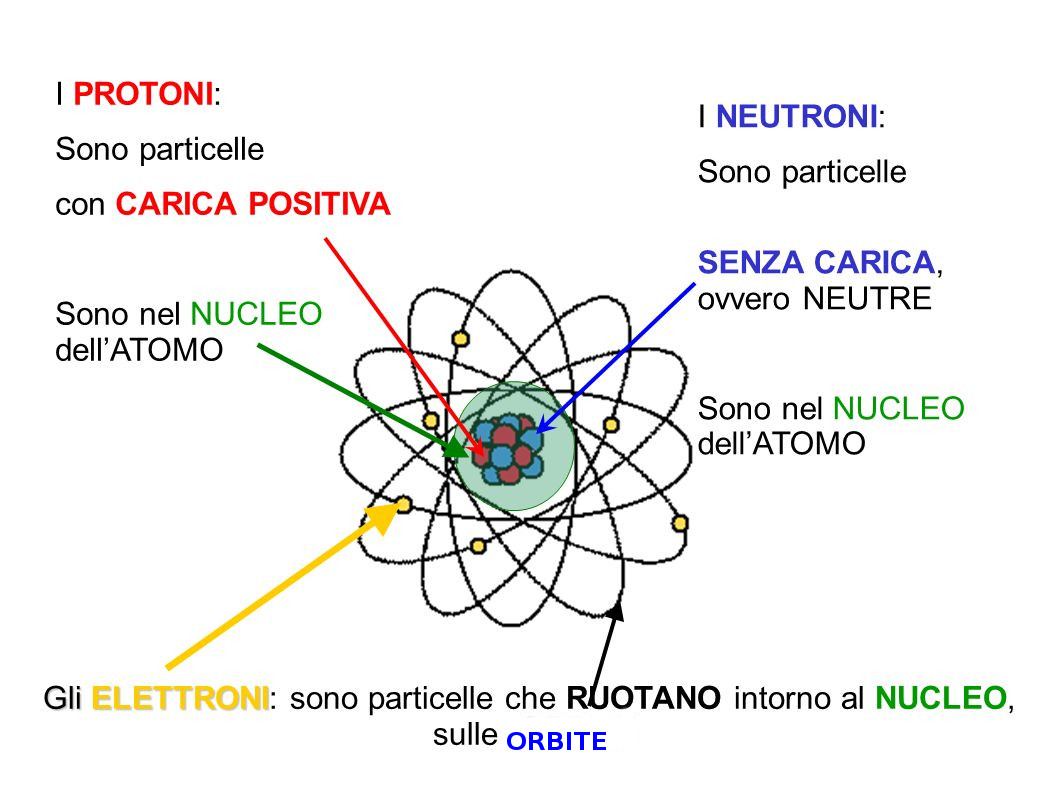
\includegraphics[width=9cm]{atomo.jpg}
			\label{fig:atomo_di_Rutherford}
		\end{figure}

	\end{frame}

	\begin{frame}[c]\frametitle{Atomo di rame}
	    \begin{columns}
			\begin{column}{0.5\textwidth}
			\begin{figure}[tb]
				\centering
				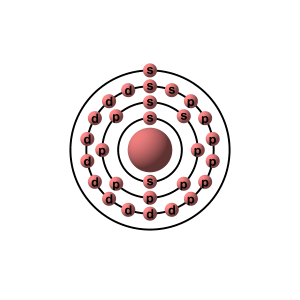
\includegraphics[width=5cm]{rame.png}
				\caption{Configurazione elettronica dell'atomo di rame (Cu)}
				\label{fig:atomo_di_rame}
			\end{figure}
			\end{column}
			\begin{column}{0.4\textwidth}
				\begin{itemize}
					\item Nucleo
					\begin{itemize}
						\item Neutroni
						\item Protoni
					\end{itemize}
					\item Elettroni
				\end{itemize}

				\vspace{0.5cm}
				
				$\longrightarrow$ Elettroni e ione!!

			\end{column}
		\end{columns}
	
	\end{frame}

	% section storia (end)

	\section{Il modello} % (fold)
	\label{sec:il_modello}
		\begin{frame}[c]\frametitle{Il metallo}
		    
		Cosa accade quando avviciniamo molti atomi?

		\begin{figure}[tb]
			\centering
			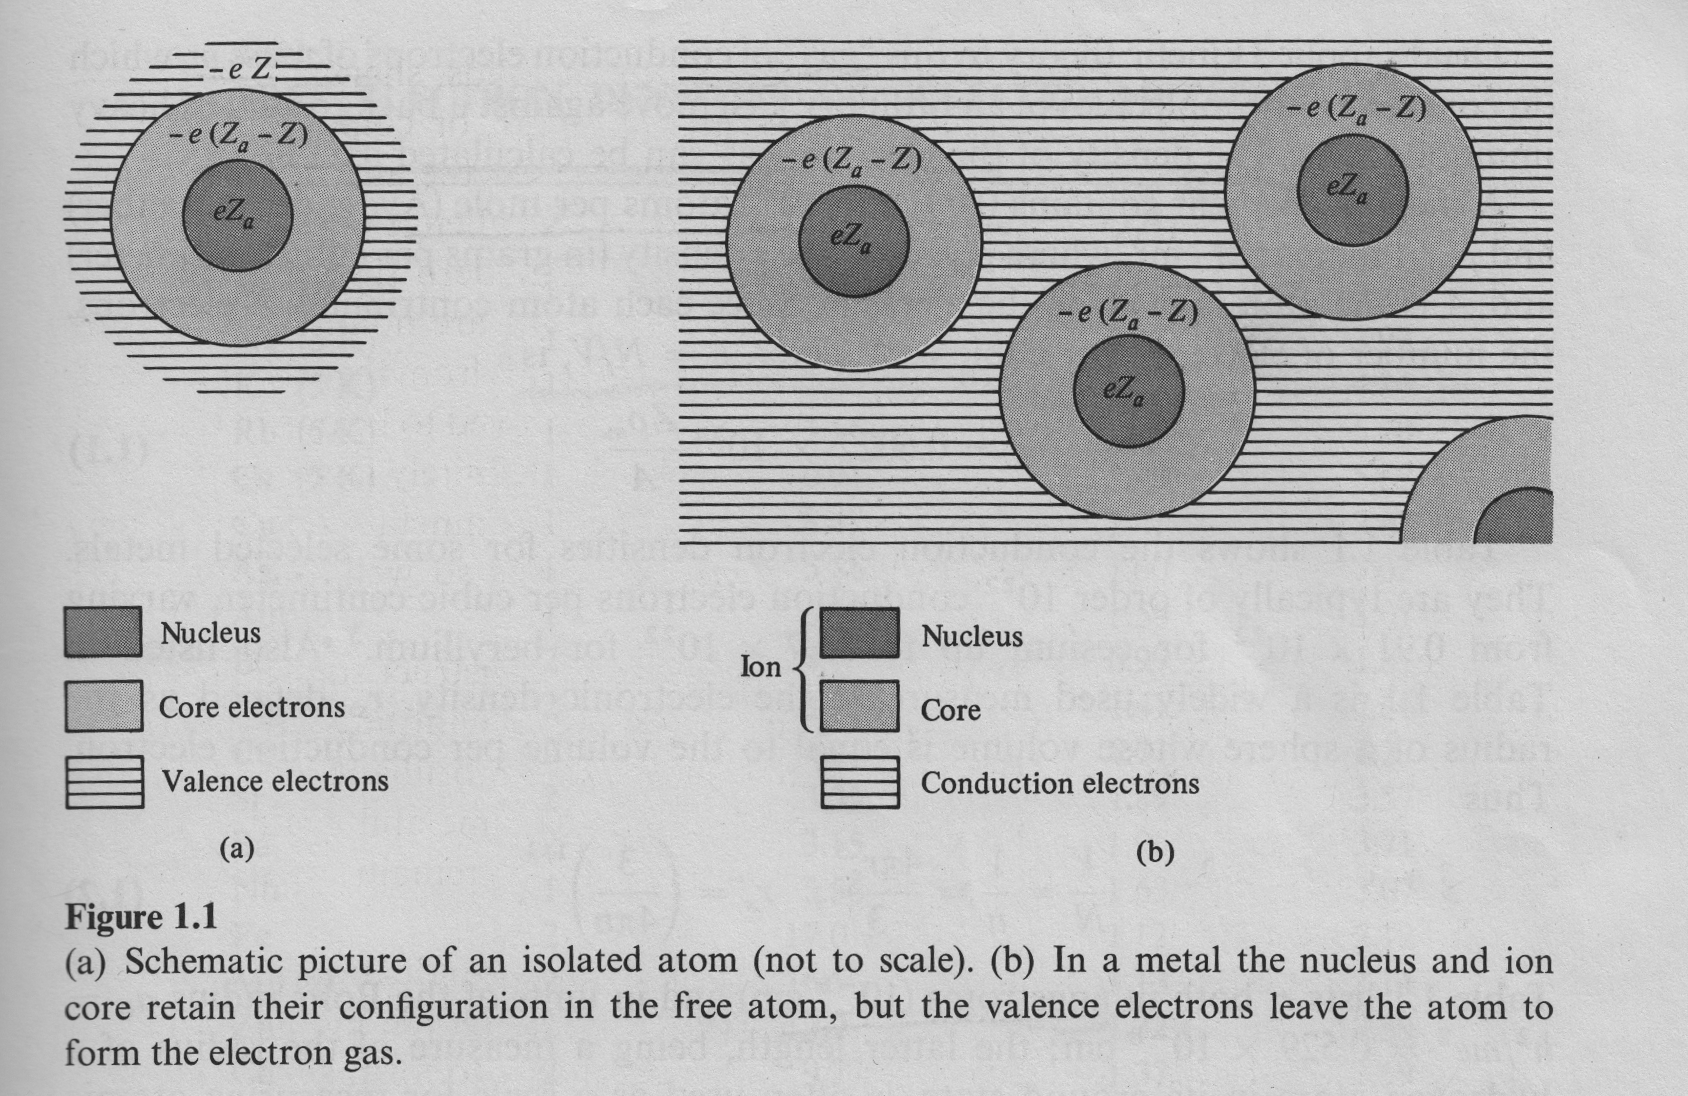
\includegraphics[width=9cm]{model.png}
			\caption{Pagina Ashcroft\/Mermin}
			\label{fig:figure1}
		\end{figure}
				
		\end{frame}
		
		\begin{frame}[c]\frametitle{Se applichiamo una differenza di potenziale?}
			\begin{columns}
				\begin{column}{0.4\textwidth}
					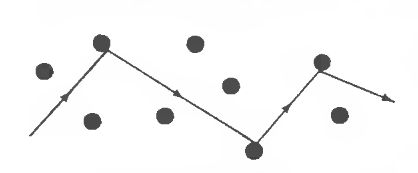
\includegraphics[width=4cm]{./img/path.png}
				\end{column}
				\begin{column}{0.7\textwidth}

					$\longrightarrow$ $V(x)$ Potenziale\\
					$\longrightarrow$ $E(x)$ Campo Elettrico
					\[
					 E (x) = - \frac{V(x1)-V(x2)}{\Delta x}
					\]
					\[
					 F \left(x\right) = q \left(x\right) E(x)
					\]

				\end{column}
			\end{columns}
			--note a mano-> convertire in slide
		\end{frame}
		\note{gli elettroni cominciano a muoversi con una direzione preferenziale }

		\begin{frame}[c]\frametitle{Disclaimer}
		    
		\begin{center}
			\color{red}\textbf{Attenzione!!}
		\end{center}
		Questo modello funziona (ovvero fa buone previsioni) su alcuni conduttori e in condizioni normali ma è FALSO, la resistenza NON è data dagli urti degli atomi con i nuclei ma fenomeni ben più complicati che richiedono conoscenze di M.Q. e di matematica non banali per essere descritti e che pertanto non andiamo ad affrontare. Abbiamo scelto questo modello perché ci è sembrato, dal punto di vista didattico il miglior modo per introdurre l'argomento.		
		\end{frame}
	% section il_modello (end)

	\section{La corrente} % (fold)
	\label{sec:la_corrente}

	\begin{frame}[c]\frametitle{La corrente}
	    
		\begin{block}{Definizione}
			asdfdasf
		\end{block}
		\[
		I = \frac{Q}{t}
		\]
	
	\end{frame}
	
	% section la_corrente (end)

	\section{La resistenza} % (fold)
	\label{sec:la_resistenza}
		\begin{frame}[c]\frametitle{Resistenza:Come si misura e come si calcola?}
		    Ma tutto quello che abbiamo visto come si porta alla quotidianità?			
		\end{frame}
		\begin{frame}[c]\frametitle{Resistenza:Come si misura e come si calcola?}
		    \begin{columns}
		    	\begin{column}{0.4\textwidth}
		    		\begin{figure}[tb]
		    			\centering
		    			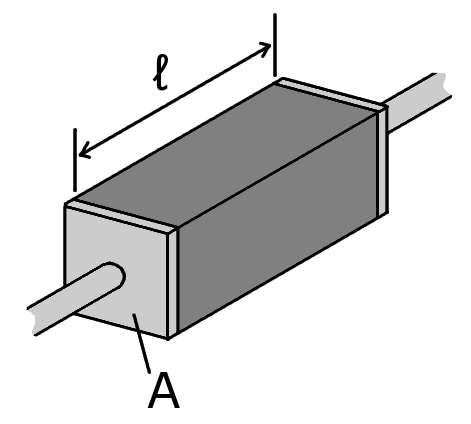
\includegraphics[width=2.5cm]{Resistivity_geometry.png}
		    			\label{fig:resistenza_resistivita}
		    		\end{figure}
		    		\[
		    		 R = \frac{\rho l}{A}
		    		\]
		    		Dove $\rho$ è in $\Omega$ per metro.\\
		    		\scriptsize{Osservazione: l'oro non conduce poi così bene, perché allora si comprano i contatti placcati in oro?}
		    	\end{column}
		    	\begin{column}{0.8\textwidth}
		    		\begin{figure}[tb]
		    			\centering
		    			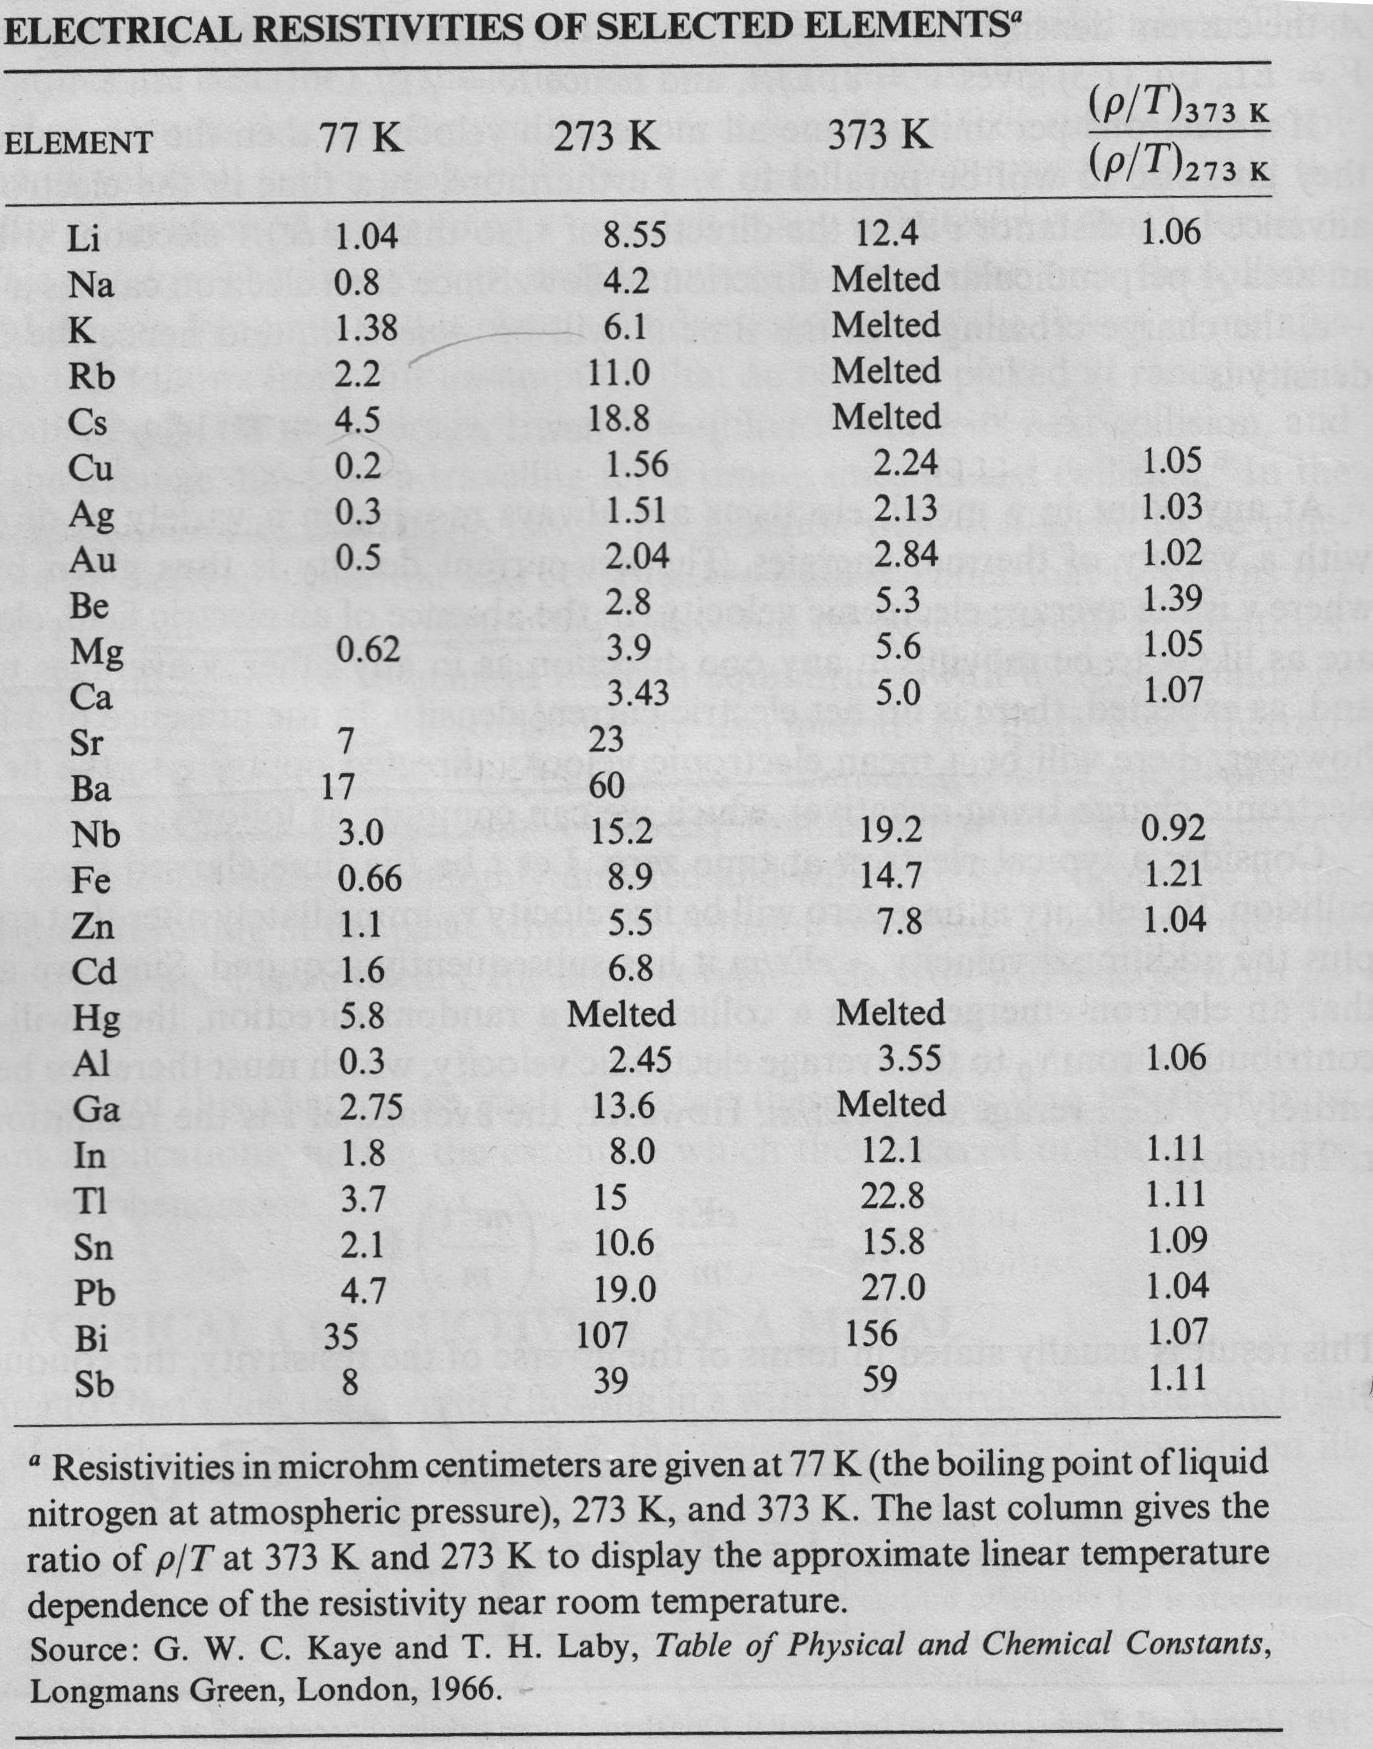
\includegraphics[width=5.5cm]{rho.jpg}
		    			\caption{A\&M}
		    			\label{fig:resistivita}
		    		\end{figure}
		    	\end{column}
		    \end{columns}	
		\end{frame}

		\begin{frame}[c]\frametitle{Resistori: come si comprano?}
		    \centering
		\begin{tabular}{c|c|c}
		Serie & Precisione & stato \\
		\hline
		E6	& 20\% & ormai rarissima  \\
		E12	& 10 \% & la più comune  \\
		E24	& 5  \% \\
		E48	& 2  \% & usata in rare applicazioni \\
		\end{tabular}
		
		\bigskip
		
		Nota: vengono vendute a pacchi da mille circa per 3-4 euro
		---- aggiungere slide sulla mappatura dello spazio -----
		
		\end{frame}

		\begin{frame}[c]\frametitle{Resistori: come si comprano?}

		\centering La serie E 12 in tutto il suo splendore, ma perché 12?
		    
		\begin{tabular}{c|c|c|c|c|c|c|c}
			1.0 & 10 & 100 & 1.0K & 10K & 100K & 1.0M & 10M \\
			1.2 & 12 & 120 & 1.2K & 12K & 120K & 1.2M & 12M \\ 
			1.5 & 15 & 150 & 1.5K & 15K & 150K & 1.5M & 15M  \\
			1.8 & 18 & 180 & 1.8K & 18K & 180K & 1.8M & 18M  \\
			2.2 & 22 & 220 & 2.2K & 22K & 220K & 2.2M & 22M  \\
			2.7 & 27 & 270 & 2.7K & 27K & 270K & 2.7M & \\
			3.3 & 33 & 330 & 3.3K & 33K & 330K & 3.3M & \\
			3.9 & 39 & 390 & 3.9K & 39K & 390K & 3.9M & \\
			4.7 & 47 & 470 & 4.7K & 47K & 470K & 4.7M & \\
			5.6 & 56 & 560 & 5.6K & 56K & 560K & 5.6M & \\
			6.8 & 68 & 680 & 6.8K & 68K & 680K & 6.8M & \\
			8.2 & 82 & 820 & 8.2K & 82K & 820K & 8.2M & \\
		\end{tabular}
		
		\end{frame}

		\begin{frame}[c]\frametitle{Resistori: come si comprano?}
		
		E se non è in nessun elenco? lo scopriamo dopo :)\\
		Piuttosto: Come le distinguiamo?\\
		
		\begin{figure}[tb]
			\centering
			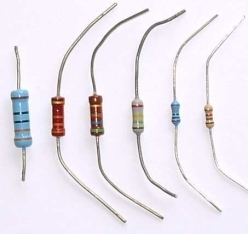
\includegraphics[width=4cm]{resistenze.jpg}
			\caption{Alcune resistenze di varia potenza}
			\label{fig:resistenze1}
		\end{figure}
		
		\end{frame}

		\begin{frame}[c]\frametitle{Resistori: come distinguono?}
			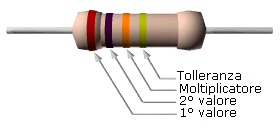
\includegraphics[width= 5cm]{r5.png}
		    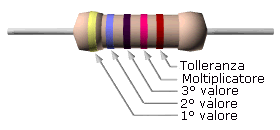
\includegraphics[width= 5cm]{r1.png}\\
		    \centering 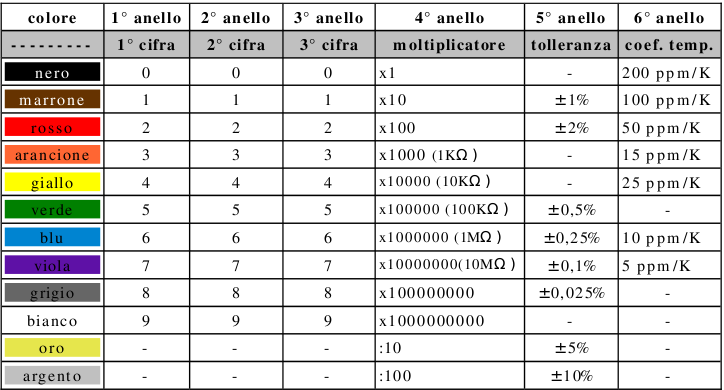
\includegraphics[width= 8cm]{codice.png}
		\end{frame}

		\begin{frame}[c]\frametitle{Resistori: La dipendenza dalla temperatura}
		    
			La resistenza aumenta all'aumentare della temperatura, ma come?
			\[
			R(T) = R_0 \left(1 + \alpha \left(T - T_0\right)\right)
			\]
			dove
			\begin{itemize}
				\item $R_0$ è la resistenza a temperatura ambiente $\si{\ohm}$
				\item $T$ è la temperatura di arrivo $\si{\celsius}$
				\item $T_0$ è la temperatura ambiente $\si{\celsius}$
				\item $\alpha$ è il coefficiente di temperatura $\si{\per\celsius}$
			\end{itemize}
		
		\end{frame}
		
		\begin{frame}[c]\frametitle{Codice dei colori, un paio di esempi}
		    \begin{figure}[tb]
		    	\centering
		    	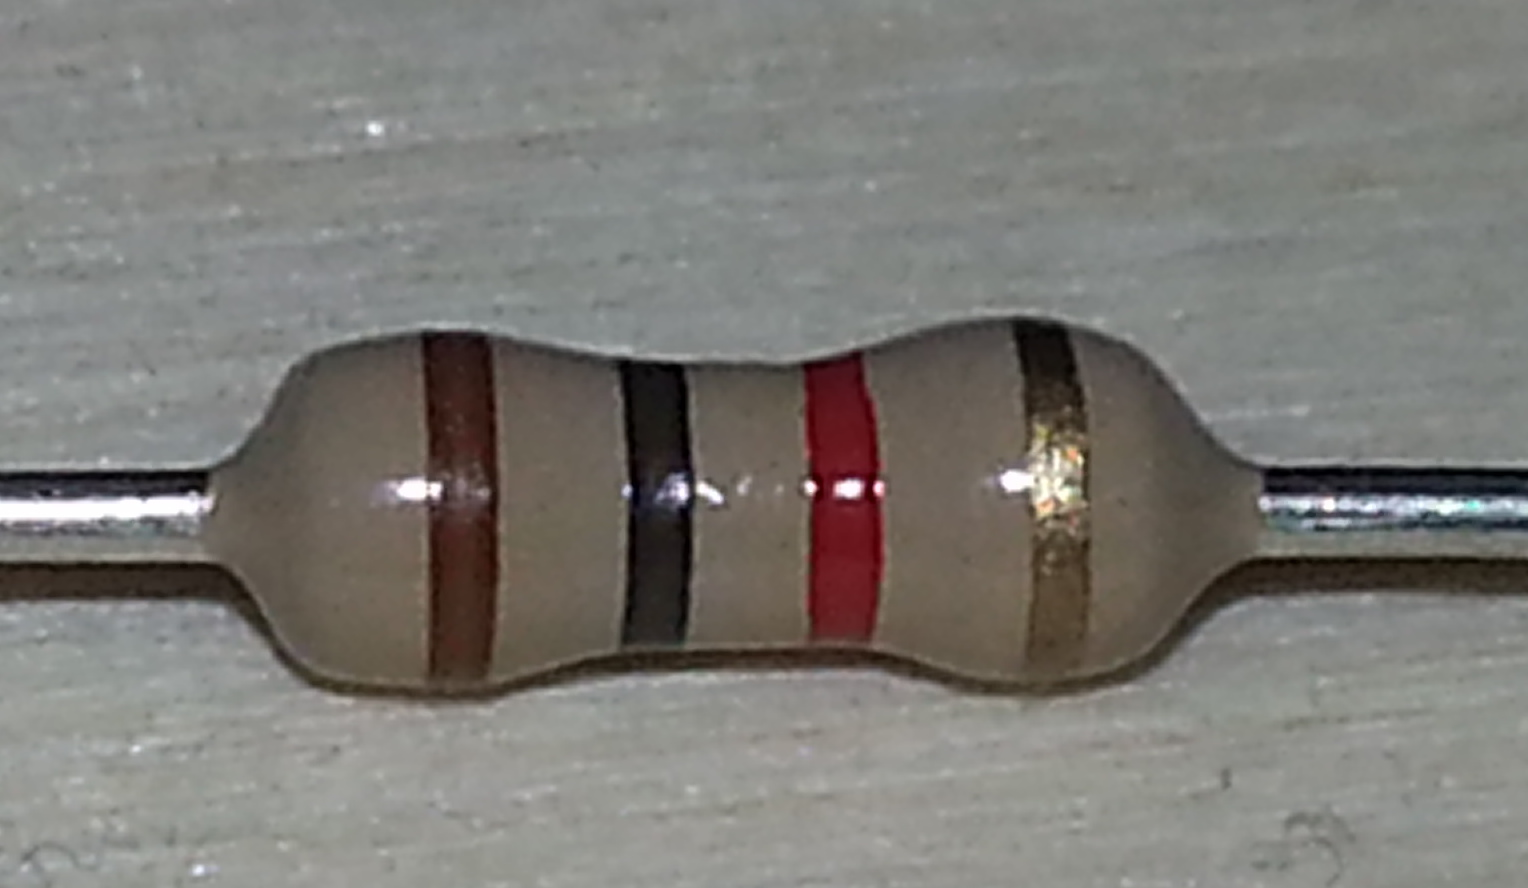
\includegraphics[width= 5 cm] {./img/E12.jpg}
		    	\label{fig:resistore_E12}
		    \end{figure}
		    \only<2>{\color{brown}{marrone} \color{black} $\longrightarrow$ 1}
		    \only<3>{\color{black}{nero} \color{black} $\longrightarrow$ 0}
		    \only<4>{\color{red}{rosso} \color{black} $\longrightarrow$ 2}
		    \only<5>{\color{yellow}{oro} \color{black} $\longrightarrow ~ \pm 5\% $}
			\[
			\only<1> {R =}
			\only<2> {R = 1 }
			\only<3> {R = 10}
			\only<4> {R = 10*10^{2}}
			\only<5> {R = 1000  \pm 5\% \si{\ohm}}
			\]
		\end{frame}

		\begin{frame}[c]\frametitle{Codice dei colori, un paio di esempi}
			\begin{figure}[tb]
				\centering
				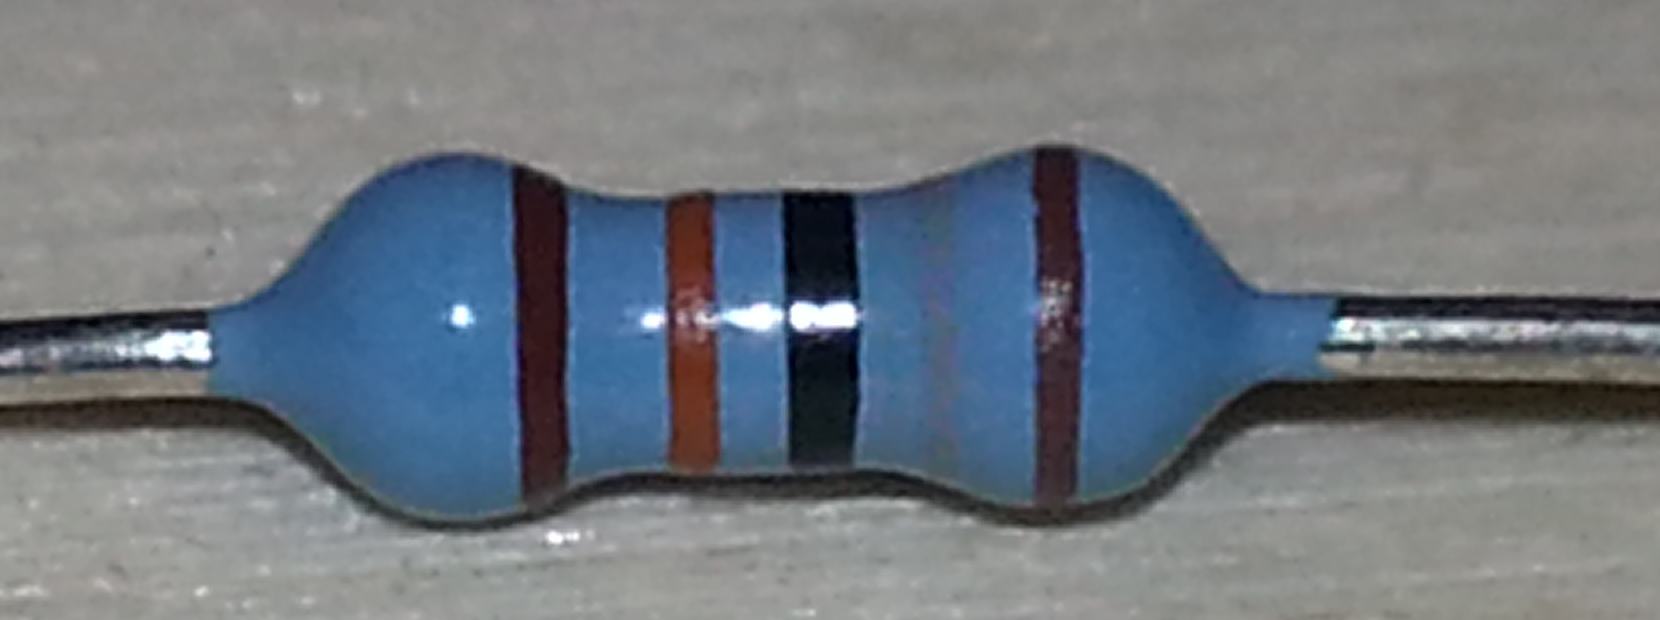
\includegraphics[width= 5 cm,angle=180] {E19.jpg}			
				\label{fig:resistore_E19}
			\end{figure}
			\only<2>{\color{brown}{marrone} \color{black} $\longrightarrow$ 1}
		    \only<3>{\color{gray}{grigio} \color{black} $\longrightarrow$ 8}
		    \only<4>{\color{black}{nero} \color{black} $\longrightarrow$ 0}
		    \only<5>{\color{orange}{arancio} \color{black} $\longrightarrow$ 3}
		    \only<6>{\color{brown}{marrone} \color{black} $\longrightarrow ~ \pm 1\% $}
			\[
			\only<1> {R =}
			\only<2> {R = 1 }
			\only<3> {R = 18}
			\only<4> {R = 180}
			\only<5> {R = 180*10^{3}}
			\only<6> {R = 180  \pm 1\% \si{\kilo\ohm}}
			\]
		\end{frame}
	% section la_resistenza (end)

	\section{La differenza di potenziale} % (fold)
	\label{sec:la_differenza_di_potenziale}
		
		\begin{frame}[c]\frametitle{DDP}
		    
			Parliamo ora della differenza di potenziale
		
		\end{frame}

		\begin{frame}[c]\frametitle{DDP: un analogia molto chiarificatrice}
		    
			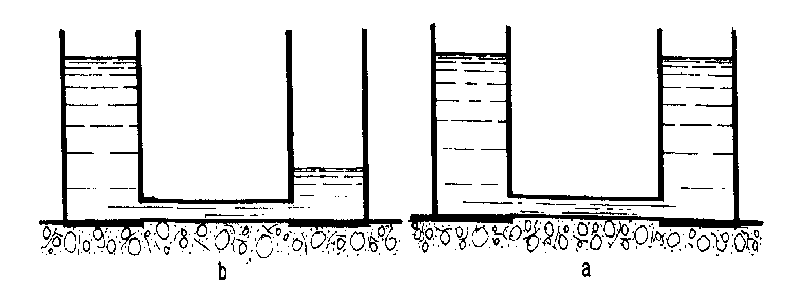
\includegraphics[width=10cm]{ddp1.png}
		
		\end{frame}

		\begin{frame}[c]\frametitle{DDP: un analogia molto chiarificatrice}
		    
			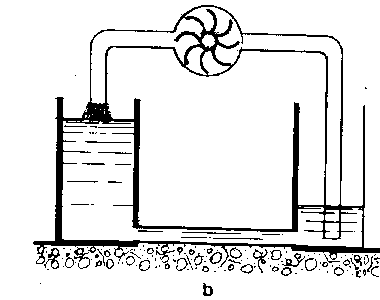
\includegraphics[width=8CM]{ddp2.png}\\

			\href{http://web.mclink.it/MK1411/Apprendistato/ImpiantiElettrici/Lezioni\%20di\%20Elettrotecnica/Lezione\%201_30_Web.htm}{Fonte}
		
		\end{frame}

		\begin{frame}[c]\frametitle{Il nostro alimentatore}
		    
			\begin{figure}[h]
				\centering
				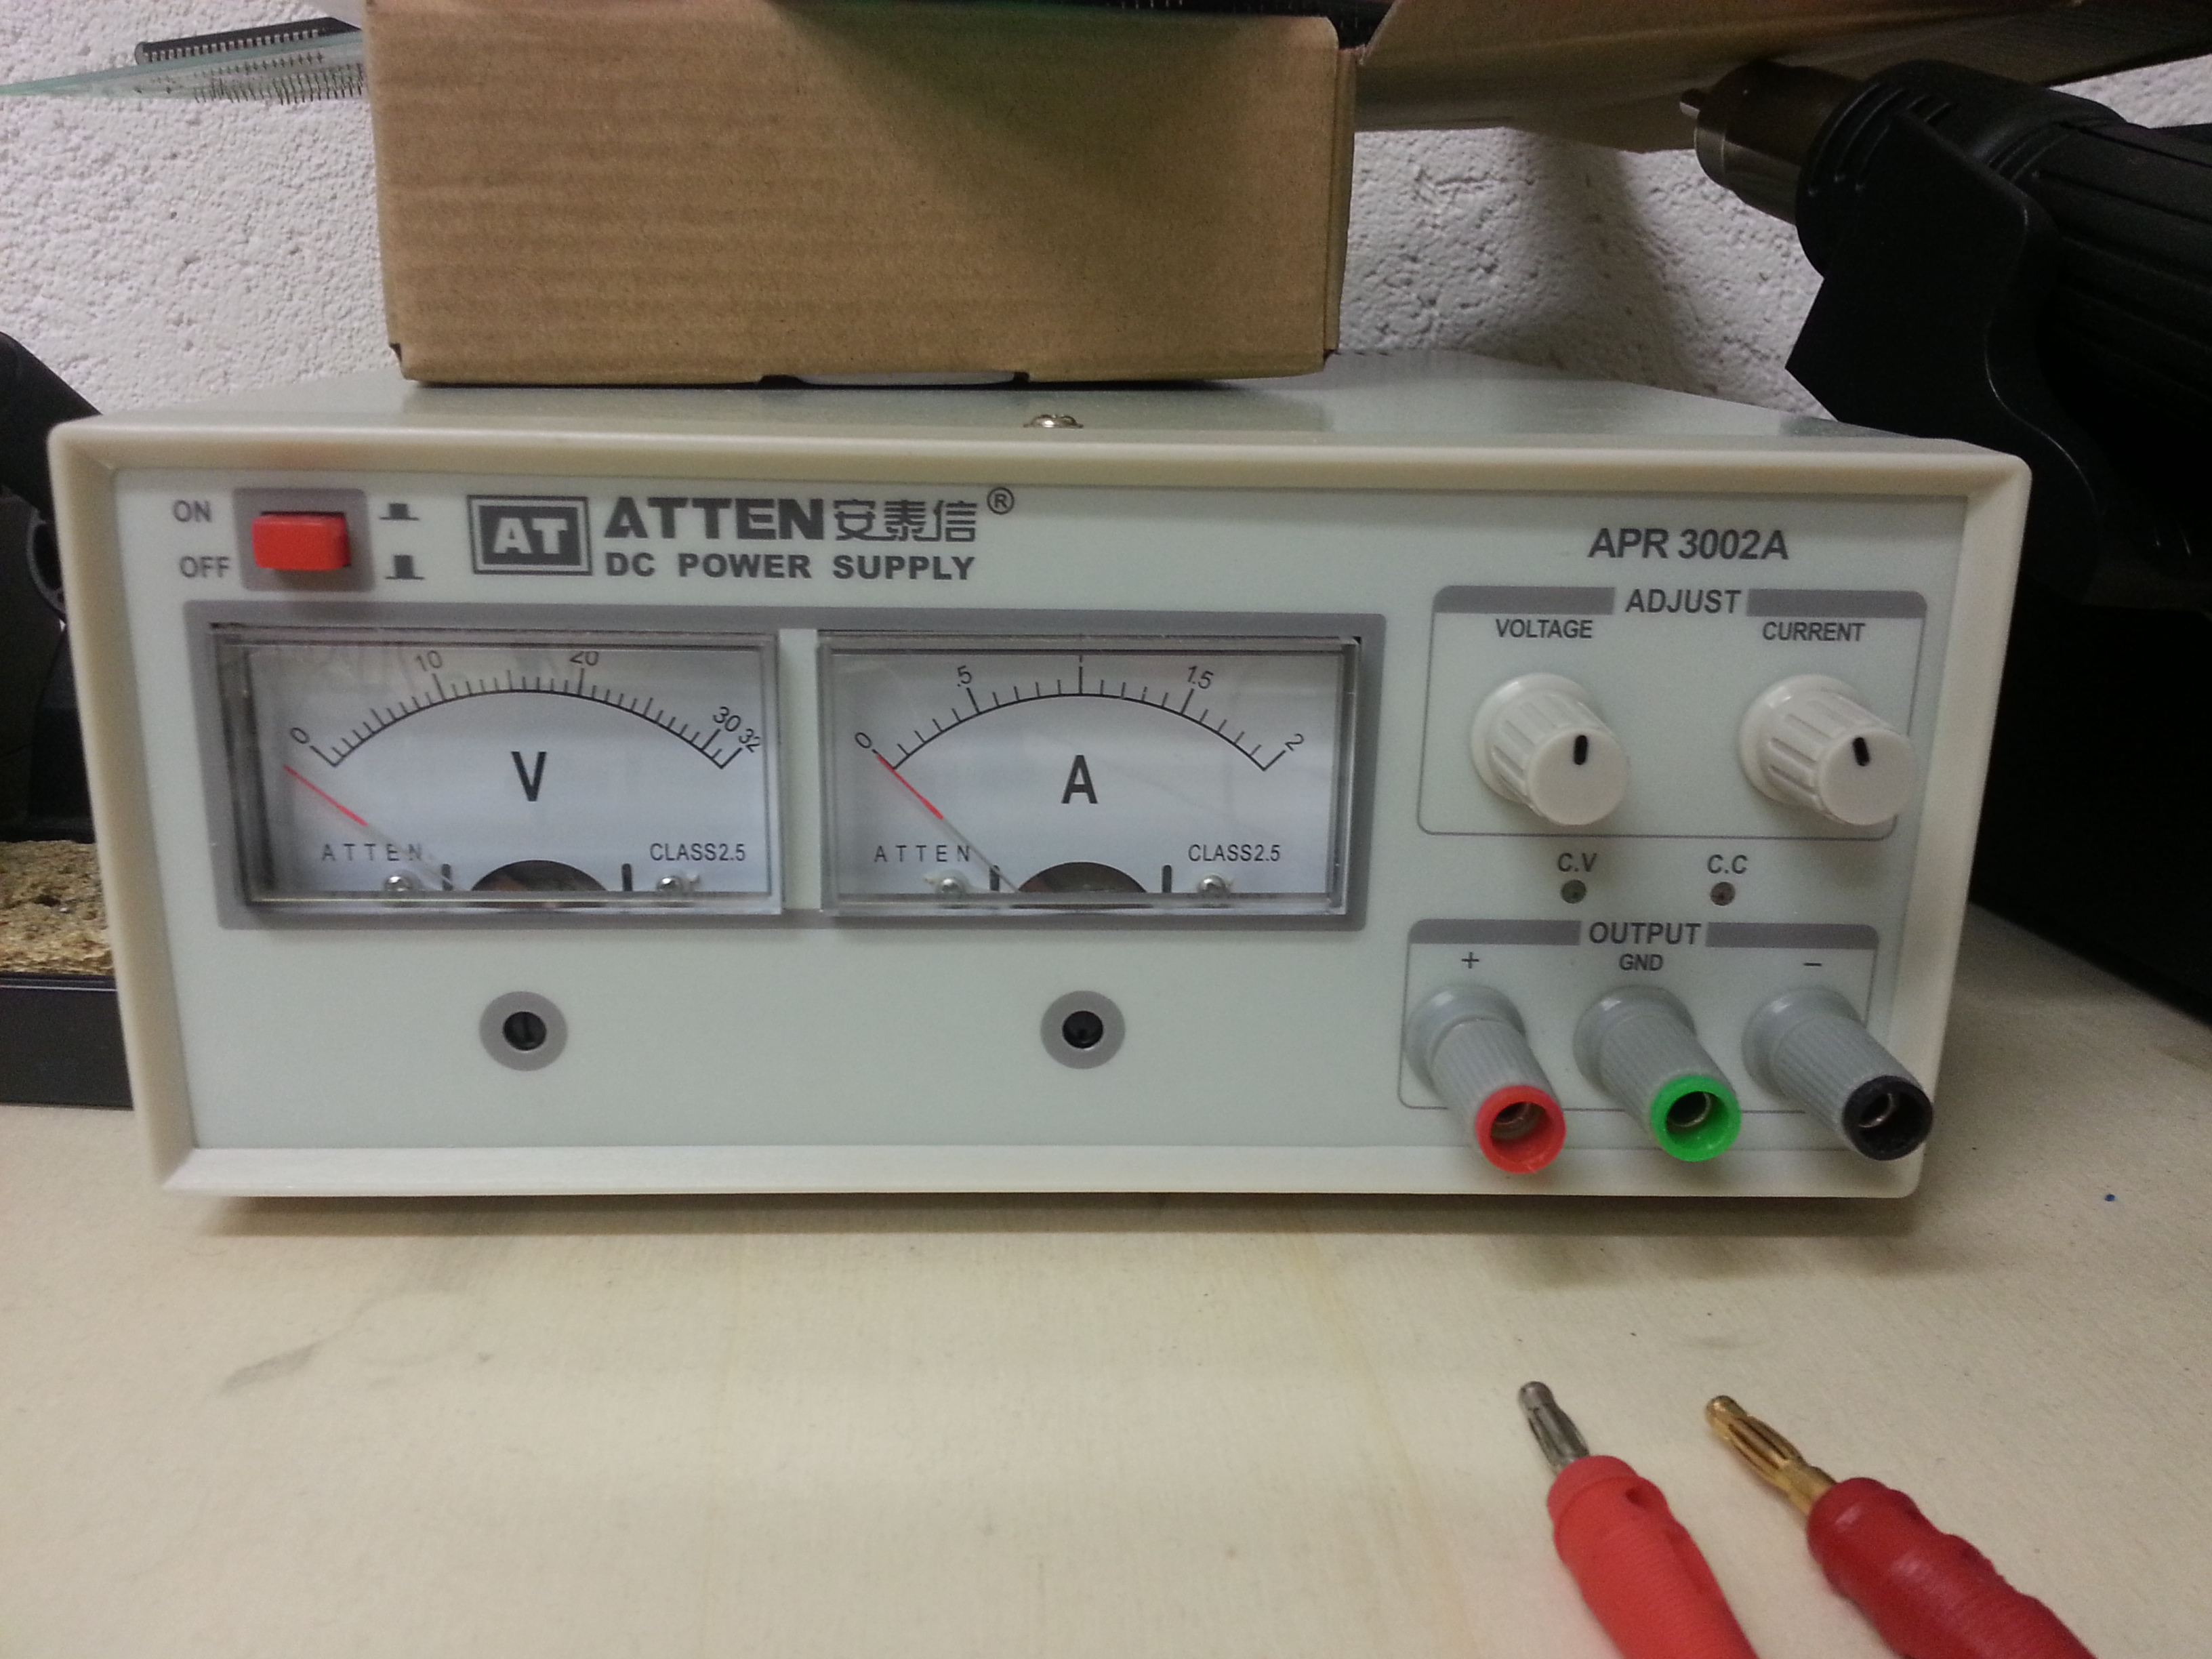
\includegraphics[width= 6cm]{alim.jpg}
				\label{fig:figure2}
			\end{figure}
			\color{red}Attenzione:
			\color{black}per prima cosa azzerare le manopole e fissare il massimo della corrente.
		
		\end{frame}

	% section la_differenza_di_potenziale (end)

	\section{La legge di OHM} % (fold)
	\label{sec:la_legge_di_ohm}
		\begin{frame}[c]\frametitle{La legge di Ohm}
		     \begin{block}{Legge di Ohm}
		     	La legge di Ohm esprime la legge costitutiva di proporzionalità diretta tra la differenza di potenziale elettrico applicata ai capi di un conduttore e l'intensità della corrente elettrica che lo attraversa. 	
		     \end{block}
			\[
				V = R \times I
			\]

			\begin{itemize}
				\pause
				\item Dove $V$ è la tensione $R$ è la resistenza e $I$ è la corrente.
				\pause
			 	\item \`E una relazione lineare
			 	\pause
			 	\item Noi non l'abbiamo dimostrata e la caliamo dal celo ma la nostra prima esperienza consisterà in una sua verifica.
			 \end{itemize} 

		\end{frame}
	% section la_legge_di_ohm (end)

	\section{Il multimetro} % (fold)
	\label{sec:il_multimetro}
		\begin{frame}[c]\frametitle{I nostri multimetri}
		    
			\begin{figure}[tb]
				\centering
				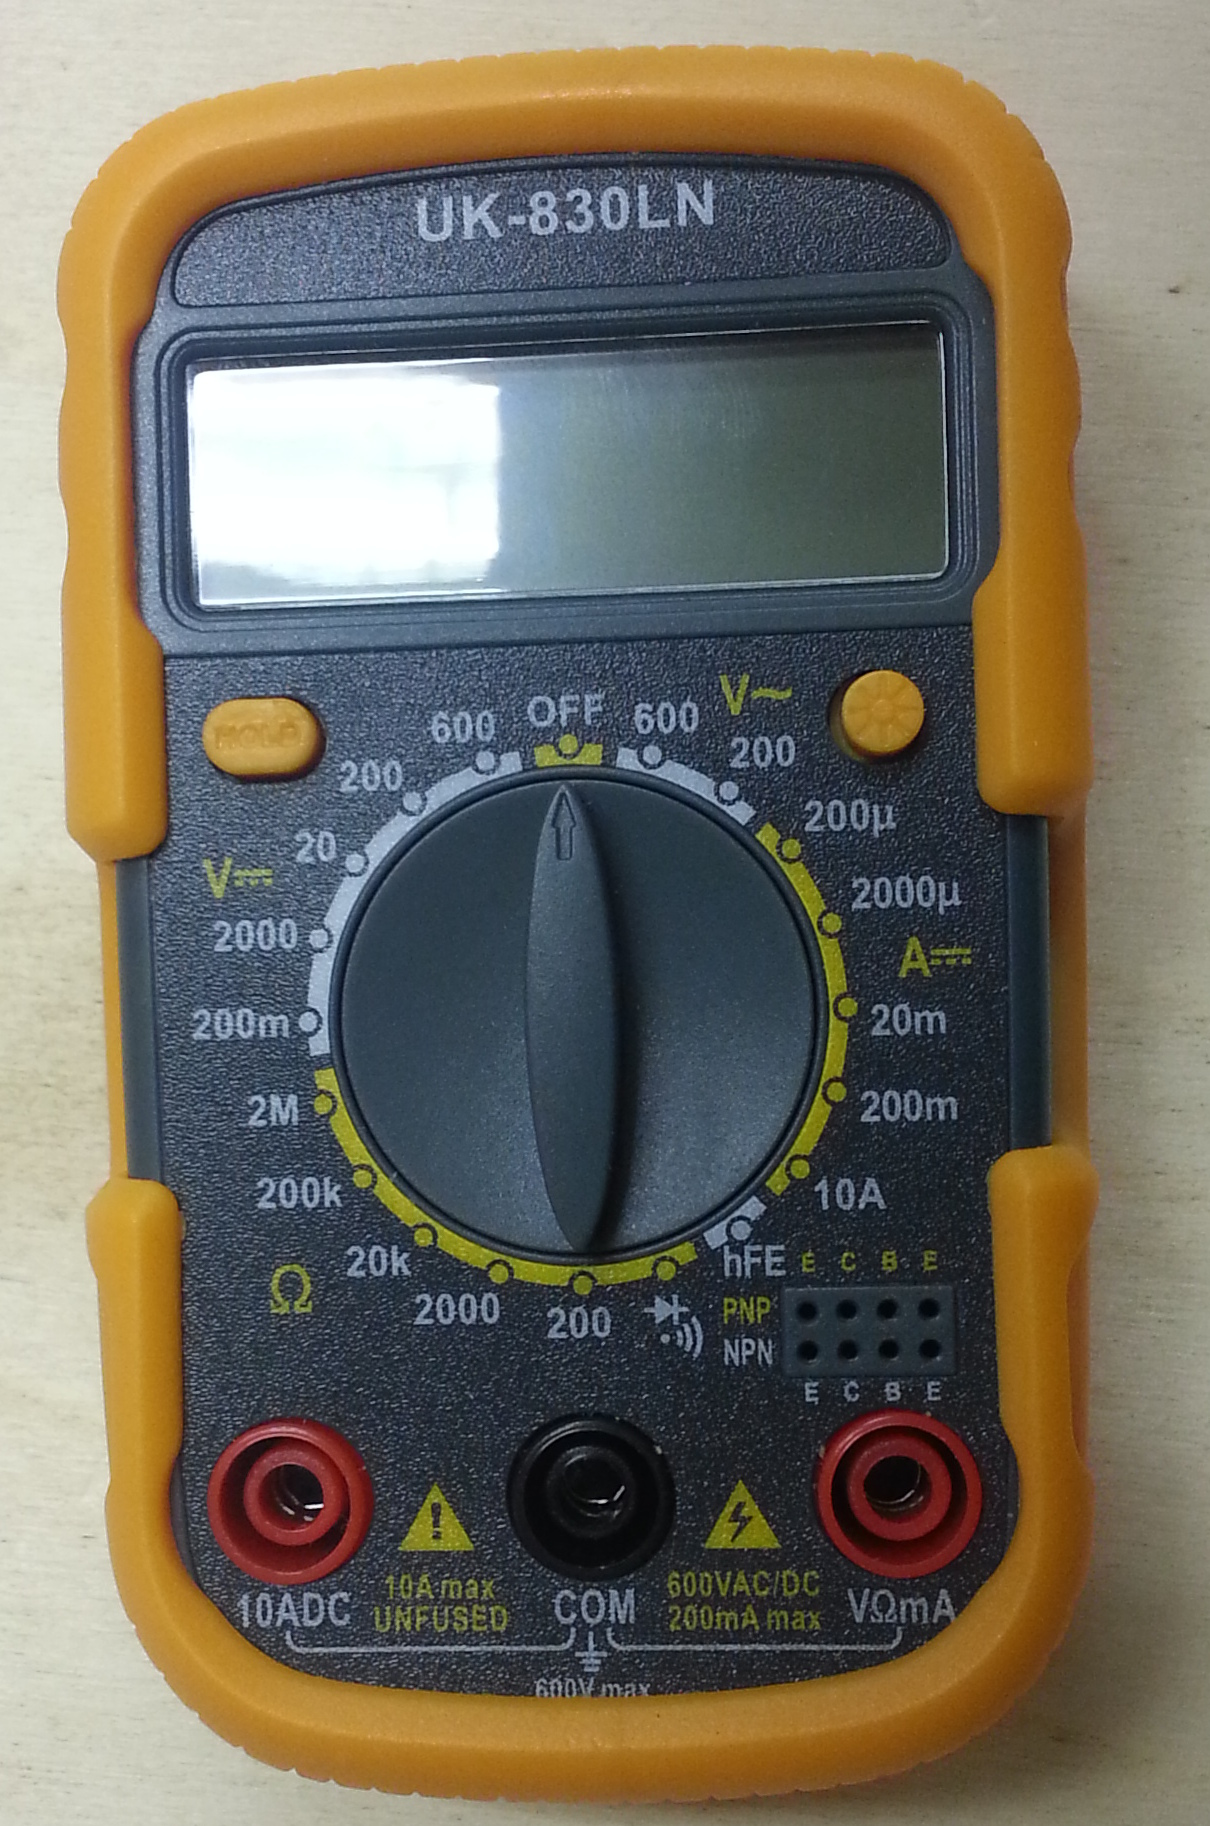
\includegraphics[width= 5cm]{./img/M_small.jpg}
				\label{fig:figure3}
			\end{figure}

			per ora non ci preoccupiamo troppo di come si collega, ve lo diciamo noi, ma appena avremmo imparato ad usare bene la legge di ohm capiremmo tutto		
		\end{frame}

		\begin{frame}[c]\frametitle{I nostri multimetri}
		    
			\begin{figure}[tb]
				\centering
				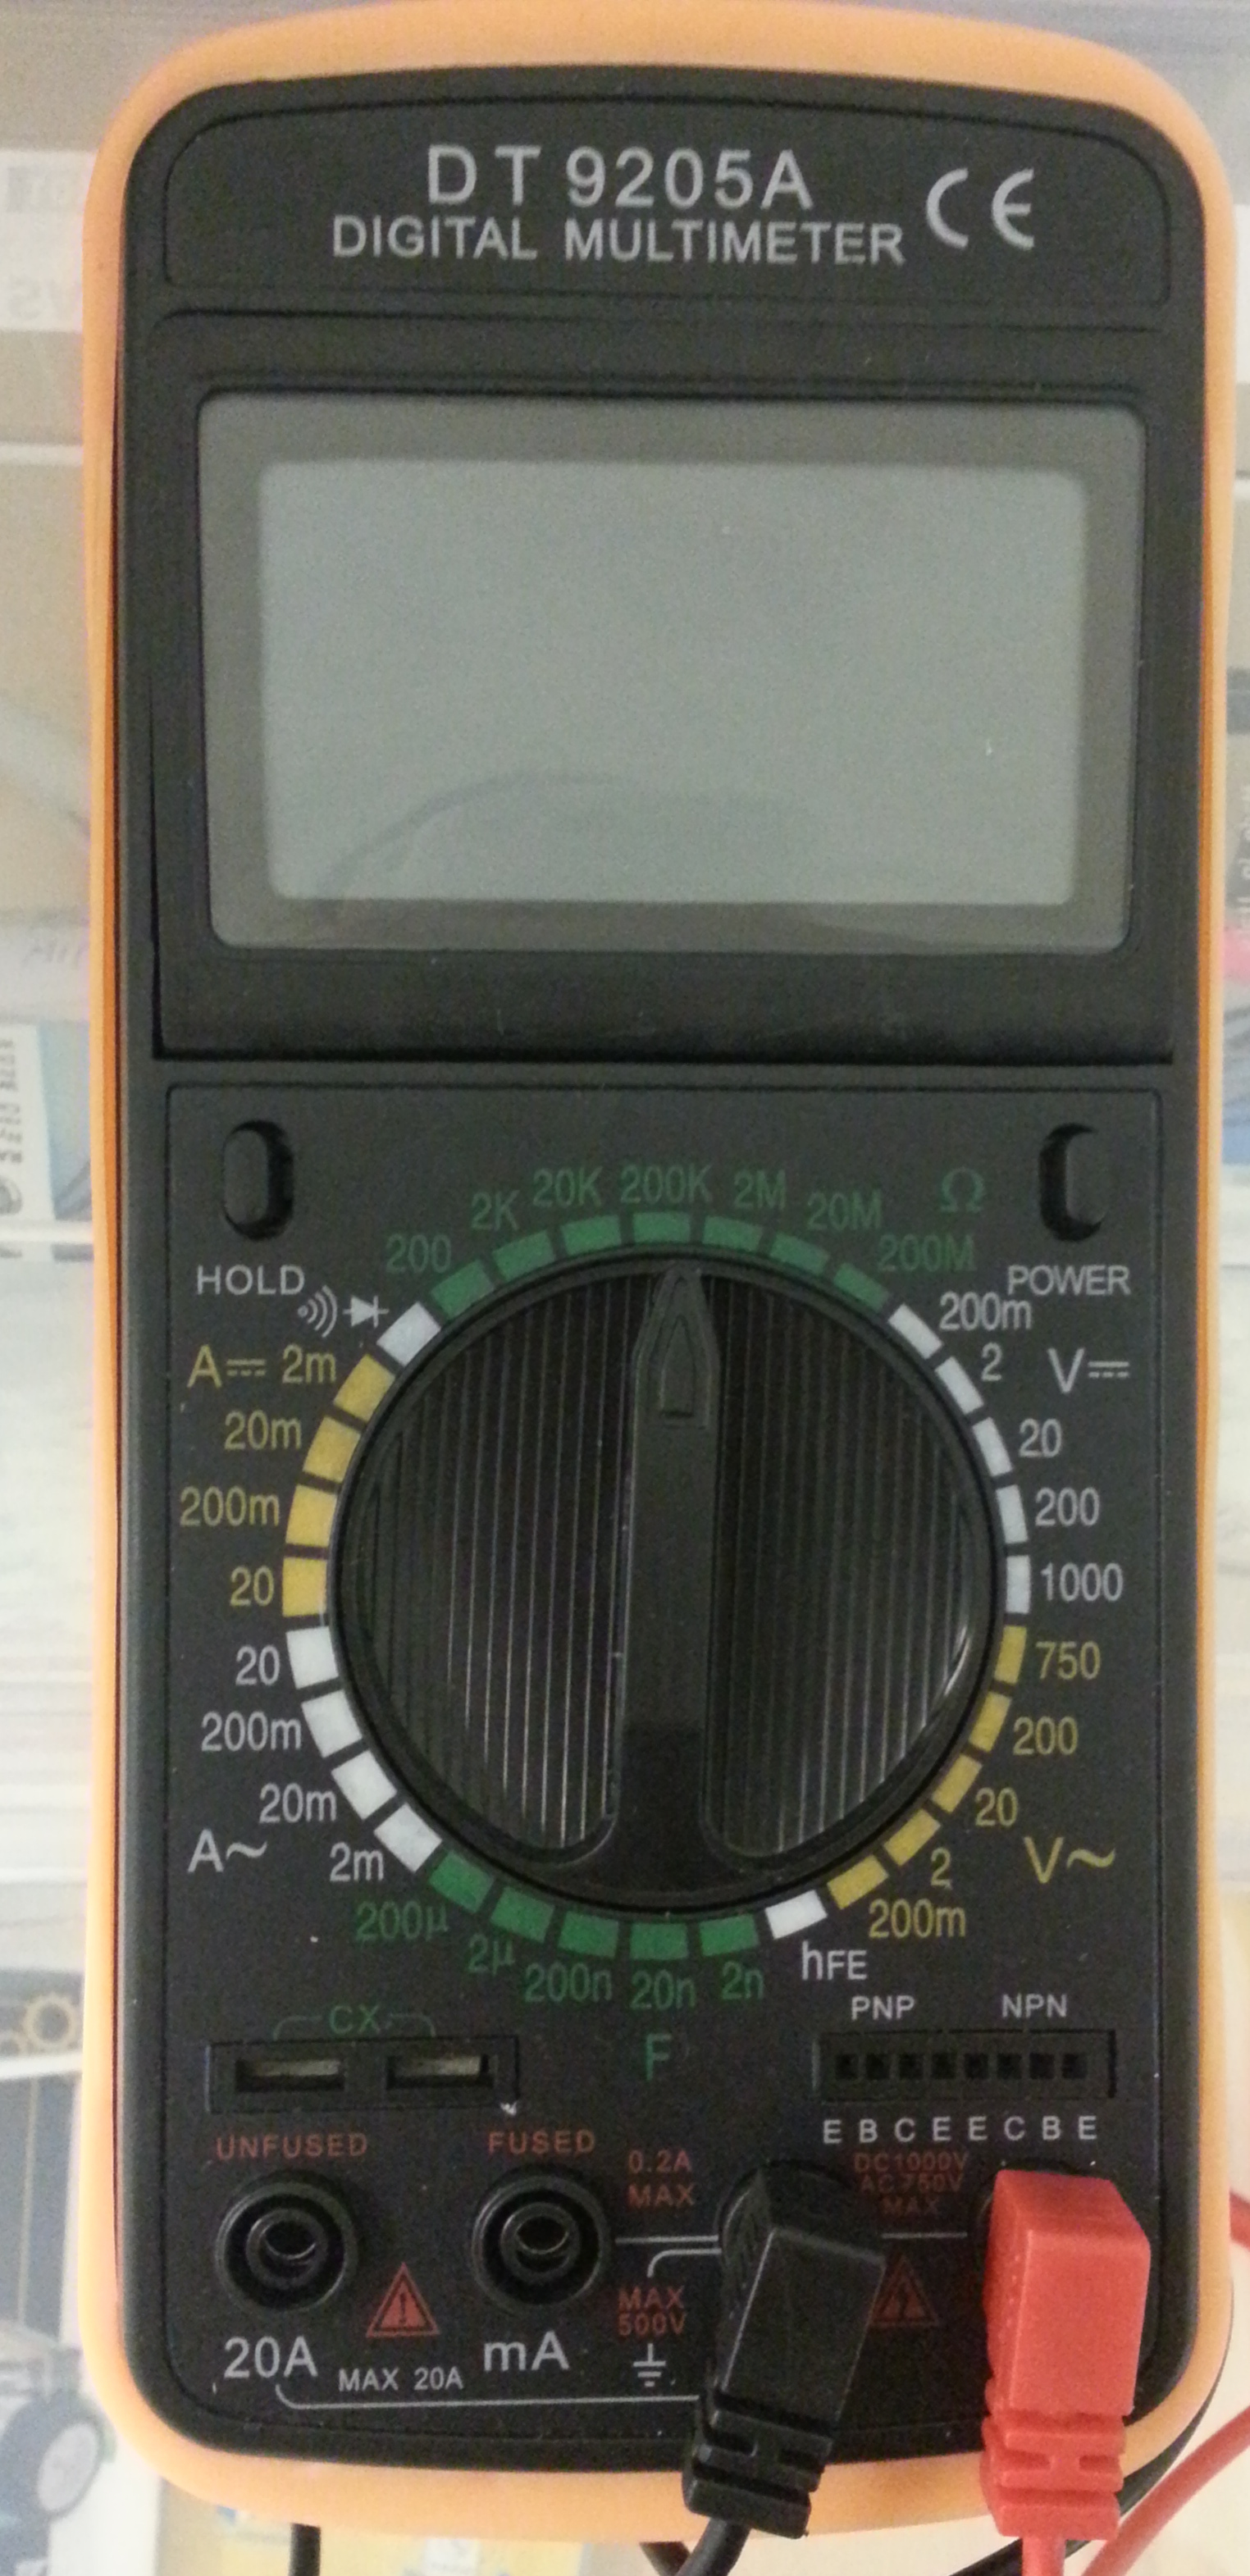
\includegraphics[width= 3.5cm]{./img/M_Big.jpg}
				\label{fig:figure3}
			\end{figure}
		
		\end{frame}
	% section il_multimetro (end)

	\section{Il nostro primo circuito} % (fold)
	\label{sec:il_nostro_primo_circuito}

		\begin{frame}[c]\frametitle{Il nostro primo circuito}
			\centering
			\begin{circuitikz} 
				\draw (0,0)
      			to[battery,v=$V_0$] (0,2) % The voltage source
     			to[short] (2,2)
      			to[R=$R$] (2,0) % The resistor
     			to[short] (0,0);
			\end{circuitikz}
		\end{frame}

		\begin{frame}[c]\frametitle{Il nostro primo circuito}
		    \centering
			\begin{circuitikz} 
			\draw (0,0)
      			to[V,v=$V_0$] (0,2) % The voltage source
     			to[short] (2,2)
      			to[R=$R$] (2,0) % The resistor
     			to[short] (0,0);
			\end{circuitikz}
		
		
		\end{frame}

		\begin{frame}[c]\frametitle{Il nostro primo circuito}
		    \centering
			\begin{circuitikz} 
			\draw (0,0)
      			to[V,v=$V_0$] (0,2) % The voltage source
     			to[ammeter] (2,2)
      			to[R=$R$] (2,0) % The resistor
     			to[short] (0,0);
     		\draw (2,2)
     			to [short] (4,2)
     			to [voltmeter] (4,0)
     			to [short] (2,0);
			\end{circuitikz}		
		\end{frame}	
	% section il_nostro_primo_circuito (end)

%%% Local Variables:
%%% mode: latex
%%% TeX-master: "slide"
%%% End:
	\section{Serie? Parallelo?}
\label{sec:serie-parallelo}
\begin{frame}
  \frametitle{Resistenza equivalente}
  Se abbiamo una rete composta solamente da resistori, è possibile sostituirli con uno soltanto?
  \begin{figure}
    \centering
    \includegraphics<1>[scale=0.39]{./img/nerd_sniping}
    \only<2>{
    \begin{tikzpicture}[circuit ee IEC,set resistor graphic=var resistor IEC graphic]
      \node[contact] (contact left) at (1,0) {};
      \node[contact] (contact middle) at (3,0) {};
      \node[contact] (contact upper right) at (5,0.5) {};
      \node[contact] (contact lower right) at (5,-0.5) {};
      \node[resistor,ohm=150] (R1) at (2,0) {};
      \node[resistor,ohm=100] (R2) at (4,0.5) {};
      \node[resistor,ohm=200] (R3) at (4,-0.5) {};
      \node[resistor,ohm'=530] (R4) at (3,-1) {};
      \node[resistor,ohm=530] (R5) at (2,1.5) {};
      \node[resistor,ohm=530] (R6) at (4,1.5) {};
      \draw (0,0) to (contact left) to (R1) to (contact middle) |- (R3.input);
      \draw (contact middle) |- (R2.input);
      \draw (contact left) |- (R5.input);
      \draw (R5) to (R6) -| (contact upper right);
      \draw (contact left) |- (R4.input);
      \draw (R2) to (contact upper right);
      \draw (R3) to (contact lower right);
      \draw (R4) -| (contact lower right);
      \draw (contact lower right) to (contact upper right) to (5.5,0.5);

      \node at (6,0.5) {$\equiv$};
      \node[resistor,ohm=?] (R) at (7,0.5) {};
    \end{tikzpicture}
    }
  \end{figure}
\end{frame}

\begin{frame}
  \Huge Iniziamo da qualcosa di più semplice\ldots
\end{frame}

\begin{frame}{Resistori in serie}
  \begin{figure}
    \centering
    \begin{tikzpicture}[circuit ee IEC,
                        set resistor graphic=var resistor IEC graphic]
      \draw<1-2> (0,0) to [resistor={ohm=100}] (3,0)
                  to [resistor={ohm=100}] (6,0);
      \draw<3-> (2,0) to [resistor={ohm=200}] (5,0);
    \end{tikzpicture}
  \end{figure}
  \begin{itemize}
  \item<1-> Cosa succede se colleghiamo due resistori in serie?
  \item<1-> Ripensate al modello di Drude\ldots
  \item<invisible@1> Se prendiamo due resistori uguali, avremo il doppio degli atomi contro cui gli elettroni collidono!
  \item<invisible@1> Quindi, la resistenza equivalente di due resistori uguali sarà\ldots
  \item<invisible@-2> \ldots{}il doppio della resistenza del singolo!
  \end{itemize}
\end{frame}

\begin{frame}{Proviamo:}
  \begin{figure}
    \centering
    \begin{tikzpicture}[circuit ee IEC, set resistor graphic= var resistor IEC graphic]
        \draw (0,4.5) to [resistor={ohm=1k}]   (3,4.5)
                      to [resistor={ohm=15k}]  (6,4.5);
        \draw (0,3)   to [resistor={ohm=2k}]   (2,3)
                      to [resistor={ohm=30k}]  (4,3)
                      to [resistor={ohm=0.2M}] (6,3);
        \draw (0,1.5) to [resistor={ohm=200}]  (2,1.5)
                      to [resistor={ohm=1k}]   (4,1.5)
                      to [resistor={ohm=300}]  (6,1.5);
        \draw (0,0)   to [resistor={ohm=100}]  (3,0)
                      to [resistor={ohm=150}]  (6,0);
      \only<2> {
        \foreach \x in {0,1.5,3,4.5} {
          \node at (6.5, \x) {$\equiv$};
        }
        \draw (7,4.5) to [resistor={ohm=16k}]  (10,4.5);
        \draw (7,3)   to [resistor={ohm=232k}] (10,3);
        \draw (7,1.5) to [resistor={ohm=1.5k}] (10,1.5);
        \draw (7,0)   to [resistor={ohm=250}]  (10,0);
      }
    \end{tikzpicture}
  \end{figure}
\end{frame}
\begin{frame}{Resistori in parallelo}
  \begin{figure}
    \centering
    \begin{tikzpicture}[circuit ee IEC, set resistor graphic=var resistor IEC graphic]
      \only<1>{
        \node[contact] (left contact) at (1,0) {};
        \node[contact] (right contact) at (4,0) {};
        \draw (0,0) to (left contact);
        \draw (left contact) to (1,0.5) to [resistor={ohm=100}] +(3,0) to (right contact); 
        \draw (left contact) to (1,-0.5) to [resistor={ohm'=100}] +(3,0) to (right contact);
        \draw (right contact) to (5,0);
      }
      \only<2>{
        \draw (0,0) to [resistor={ohm=50}] (3,0);
      }
    \end{tikzpicture}
  \end{figure}
  \begin{itemize}
    \begin{overlayarea}{\textwidth}{3cm}
        \only<1>{\item È come se avessimo un resistore, ma due volte più ``grosso''! Quindi\ldots}
        \only<2>{\item \ldots{}due resistori uguali in parallelo avranno una resistenza equivalente pari alla metà di quella del singolo resistore!
        \begin{eqnarray*}
            \frac{1}{R} =& \frac{1}{R_1} + \frac{1}{R_2} \\
                        =& \frac{R_1 R_2}{R_1 + R_2}
        \end{eqnarray*}
      }
      \end{overlayarea}
    \end{itemize}
\end{frame}
\begin{frame}
  \frametitle{Facciamo un pò di pratica\ldots}
  \begin{figure}[ht]
    \centering
     \begin{tikzpicture}[circuit ee IEC, set resistor graphic=var resistor IEC graphic]
       \foreach \y/\contact in {0/1,2/2,4.5/3}
       {
         \node[contact] (left contact \contact) at (1,\y) {};
         \node[contact] (right contact \contact) at (4,\y) {};
         \draw (0,\y) to (left contact \contact);
         \draw (right contact \contact) to (5,\y);
         \node<2> at (5.5,\y) {$\equiv$};
       }
        \draw (left contact 1) to (1,0.5) to [resistor={ohm=450}] +(3,0) to (right contact 1); 
        \draw (left contact 1) to (1,-0.5) to [resistor={ohm=150}] +(3,0) to (right contact 1);
        \draw (left contact 2) to (1,1.5) to [resistor={ohm=420}] +(3,0) to (right contact 2);
        \draw (left contact 2) to (1,2.5) to [resistor={ohm=10k}] +(3,0) to (right contact 2);
        \draw (left contact 3) to (1,3.5) to [resistor={ohm=400}] +(3,0) to (right contact 3);
        \draw (left contact 3) to (1,4.5) to [resistor={ohm=400}] +(3,0) to (right contact 3);
        \draw (left contact 3) to (1,5.5) to [resistor={ohm=300}] +(3,0) to (right contact 3);
        \only<2> {
          \draw (6,0) to [resistor={ohm=112.5}] +(3,0);
          \draw (6,2) to [resistor={ohm=403.1}] +(3,0);
          \draw (6,4.5) to [resistor={ohm=120}] +(3,0);
        }
     \end{tikzpicture}
   \end{figure}
\end{frame}

\begin{frame}{E ora\ldots tutto insieme!}
  \begin{alertblock}{Importante!}
    Purtroppo non c'è una regola fissa per risolvere circuiti misti (non si può fare prima tutto parallelo o prima tutto in serie). Bisogna analizzare il circuito che abbiamo di fronte e semplificarlo un ``livello'' per volta.
    \begin{itemize}
    \item Si parte dalla spira più ``interna''
    \item si procede man mano verso l'esterno
    \end{itemize}
  \end{alertblock}
\end{frame}

\begin{frame}
  \frametitle{Torniamo al circuito visto prima\ldots}
  \begin{figure}
    \centering
    \begin{tikzpicture}[circuit ee IEC,set resistor graphic=var resistor IEC graphic]
      \node<-3>[contact] (contact left) at (1,0) {};
      \node<1>[contact] (contact middle) at (3,0) {};
      \node<1>[contact] (contact upper right) at (5,0.5) {};
      \node<1>[contact] (contact lower right) at (5,-0.5) {};
      \node<2-3>[contact] (contact right) at (5,0) {};

      \node<1-2>[resistor,ohm=150] (R1) at (2,0) {};
      \node<1>[resistor,ohm=100] (R2) at (4,0.5) {};
      \node<1>[resistor,ohm=200] (R3) at (4,-0.5) {};
      \node<2>[resistor,ohm=?] (R23) at (4,0) {};
      \node<3>[resistor,ohm=?] (R123) at (3,0) {};
      \node<-3>[resistor,ohm'=530] (R4) at (3,-1) {};
      \node<1-2>[resistor,ohm=530] (R5) at (2,1.5) {};
      \node<1-2>[resistor,ohm=530] (R6) at (4,1.5) {};
      \node<3>[resistor,ohm=?] (R56) at (3,1.5) {};

      \draw<1-2> (contact left) to (R1);
      \draw<3> (contact left) to (R123) to (contact right);

      \draw<1> (R1) to (contact middle) |- (R3.input);
      \draw<1> (contact middle) |- (R2.input);
      \draw<2> (R1) to (R23) to (contact right);

      \draw<-2> (contact left) |- (R5.input);
      \draw<-2> (R5) to (R6);
      \draw<3> (contact left) |- (R56) -| (contact right);

      \draw<1> (R6) -| (contact upper right);
      \draw<2> (R6) -| (contact right);
      \draw<-3> (contact left) |- (R4.input);
      \draw<2> (R4) -| (contact right);

      \draw<1> (R2) to (contact upper right);
      \draw<1> (R3) to (contact lower right);
      \draw<1> (R4) -| (contact lower right);
      \draw<3> (R4) -| (contact right);

      % Extremities
      \draw<-3> (0,0) to (contact left);
      \draw<1> (contact lower right) to (contact upper right) to (5.5,0.5);
      \draw<2-3> (contact right) to (5.5, 0);
      
      \draw<4> (0,0) to [resistor={ohm=?}] (5.5,0);

    \end{tikzpicture}
  \end{figure}
\end{frame}

\section{Kirchhoff}
\label{sec:kirchoff}
\begin{frame}
  \frametitle{Ma perché è cosi?}
  \begin{itemize}
    \item Dev'esserci una legge che governa come si comportano le correnti e le tensioni all'interno di un circuito.
    \item Infatti c'è: le due leggi ti Kirchhoff!
      \begin{itemize}
        \item Legge di Kirchhoff per le tensioni
        \item Legge di Kirchhoff per le correnti
      \end{itemize}
      \item Vediamole in dettaglio\ldots
  \end{itemize}
\end{frame}

\subsection{Kirchhoff per le tensioni}
\label{subsec:kirchhoff_per_le_tensioni}

\begin{frame}
  \frametitle{La spira!}
  \begin{itemize}
    \item Definita come un circuito ``chiuso''
    \item Percorso che ritorna al punto di partenza
  \end{itemize}
  \begin{figure}
    \centering
    \begin{tikzpicture}[circuit ee IEC,set resistor graphic=var resistor IEC graphic]
      \draw (0,0) to [voltage source={info=V1}] (0,2) to [resistor={info=R1}] (2,2) to [resistor={info=R2}] (2,0) to [voltage source={info=V2}] (0,0);
    \end{tikzpicture}
  \end{figure}
\end{frame}
\begin{frame}
  \frametitle{Legge delle tensioni}
  \begin{block}{Eccola qui:}
    La somma di tutte le cadute di potenziale lungo una spira è uguale a 0.
  \end{block}
  \begin{figure}
    \centering
    \begin{tikzpicture}[circuit ee IEC,set resistor graphic=var resistor IEC graphic]
      \draw (0,0) to [voltage source={direction info={->,volt=5}}] (0,2) to [resistor={ohm=100}] (2,2) to [resistor={ohm=2k}] (2,0) to [voltage source={direction info={->,volt=2}}] (0,0);
    \end{tikzpicture}
  \end{figure}
\end{frame}

\subsection{Kirchhoff per le correnti}
\label{subsec:kirchhoff_per_le_correnti}
\begin{frame}
  \frametitle{Il nodo}
  \begin{block}{Definizione}
    Il nodo è un punto nel circuito dove si congiungono tre o più linee.
  \end{block}
  \begin{figure}[ht]
    \centering
    \begin{tikzpicture}[circuit ee IEC,set resistor graphic=var resistor IEC graphic]
      \node [contact] (contact) at (0,0) {};
      \draw (-1,0) to [current direction={info=$I_1$}] (contact) to [current direction={info=$I_3$}] (1,0);
      \draw (0,1) to [current direction'={near start, info=$I_2$}] (contact);
    \end{tikzpicture}
  \end{figure}
\end{frame}

\begin{frame}
  \frametitle{La legge delle correnti}
  \begin{block}{Enunciato}
    La somma di tutte le correnti entranti (e uscenti) in un nodo è uguale a 0.
    \[ I_1 + I_2 + I_3 = 0 \]
  \end{block}
  \begin{figure}[ht]
    \centering
    \begin{tikzpicture}[circuit ee IEC,set resistor graphic=var resistor IEC graphic]
      \node [contact] (contact) at (0,0) {};
      \draw (-1,0) to [current direction={info=$I_1$}] (contact) to [current direction={info=$I_3$}] (1,0);
      \draw (0,1) to [current direction'={near start, info=$I_2$}] (contact);
    \end{tikzpicture}
  \end{figure}
\end{frame}

\begin{frame}[c]\frametitle{Il multimetro}
    
  Perché lo avevamo collegato così nella prima esperienza?

\end{frame}

\begin{frame}
  \Huge E ora un po' di pratica\ldots
\end{frame}

%%% Local Variables:
%%% mode: latex
%%% TeX-master: "slide"
%%% End:

\end{document} 